\chapter{Conclusion and Future Work}
\section{Conclusion}
In current phase of SBN development, objectives mainly consist of following activities: 1)diagnose and refurbish individual components of the network; 2)investigate power supply system to enhance robustness; 3)design and deploy low power routers; 4)log and document these activities for future reference. We are able to identify existing problems within the system and to achieve a comprehensive understanding of local condition.
\section{Future Work}
\subsection{Routability}
Public IP addresses of a /24 network are allocated to SBN. Although, as a broadband island, this network is behind NAT while exposing few IPs assigned by ISP, as depicted in Figure \ref{nat}.
\begin{figure}[htbp]
\centering
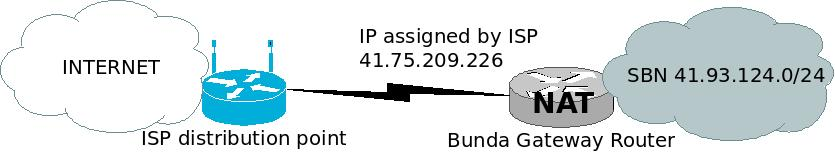
\includegraphics[width=\textwidth]{nat.jpeg}
\caption{SBN /24 network behind NAT}
\label{nat}
\end{figure}
However, global routability is desired to for necessary service being accessible from outside of SBN domain. To achieve this, three approaches are proposed.
\begin{itemize}
\item GRE Tunnel\\
IP addresses of 41.93.124.0/24 are hold by African Network Information Center (AFRINIC) and managed by TERNET. Routability can be achieved by linking broadband island to another TERNET entity which is capable of advertising the route. A complete plan can be found in Figure \ref{tunnel}. Traffic for 41.93.124.0/24 is routed to 41.93.124.1 via GRE tunnel between Bunda gateway router and TERNET gateway router.
\begin{figure}[htbp]
\centering
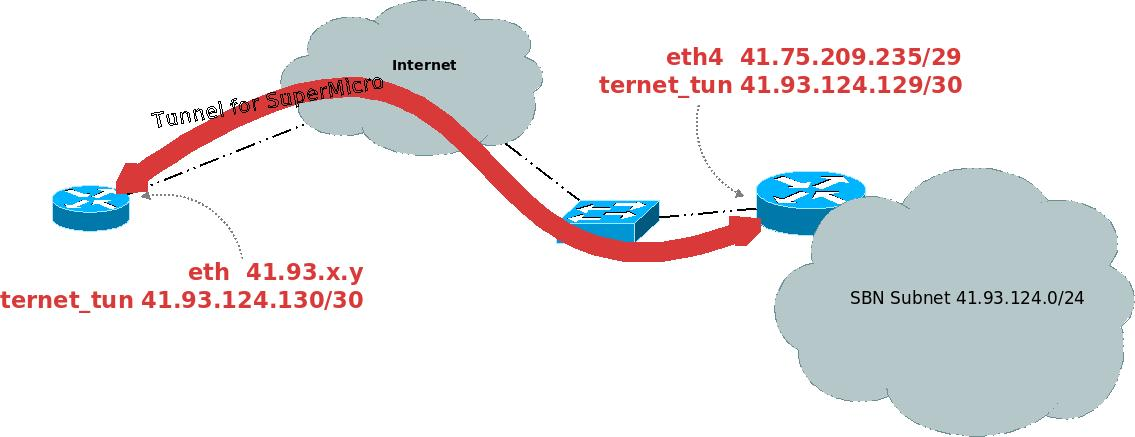
\includegraphics[width=\textwidth]{tunnel.jpeg}
\caption{GRE tunnel between TERNET gateway and SBN Bunda gateway}
\label{tunnel}
\end{figure}
\item Local ISP\\
Let the ISP be reponsible for the provision of routability, more specifically, advertising 41.93.124.0/24 network at their BGP router. This approach is the most intuitive and natural one, although it requires negotiation with ISP and might cause harmful traffic storm if misconfigured. On the other hand, two ISPs are available and there exists possibilities of switching back and forth. Therefore, this solution is not as flexible as previous one.
\item Port Forwarding\\
Port forwarding is the most lightweight and cheapest solution, which is currently being used in SBN. By adding proper iptables rules to Bunda gateway router, internal services could be accessed by requesting gateway address on specific port. However it should only be considered as a temporary solution, for it is hard to manage and not scalable.
\end{itemize}

\subsection{Wireless distribution restructure}
while distributing the network from fiber line to end-users, wireless signal is relayed by an antenna on geographic high point to obtain better coverage. A typical setting is shown in Figure \ref{wds}. Three radioes are all configured to operate in Wireless Distribution System (WDS) mode\footnote{http://wiki.openwrt.org/doc/howto/clientmode}, however the bandwidth in this scenario is halved when two wireless hops exist in between.

\begin{figure}[htbp]
\centering
\begin{subfigure}{0.45\textwidth}
\centering
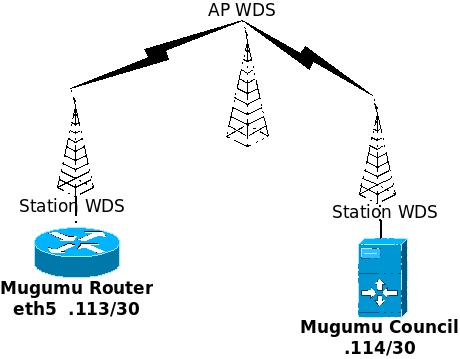
\includegraphics[width=\textwidth]{wds.jpeg}
\caption{Wireless Distribution System at Mugumu}
\label{wds}
\end{subfigure}
\begin{subfigure}{0.45\textwidth}
\centering
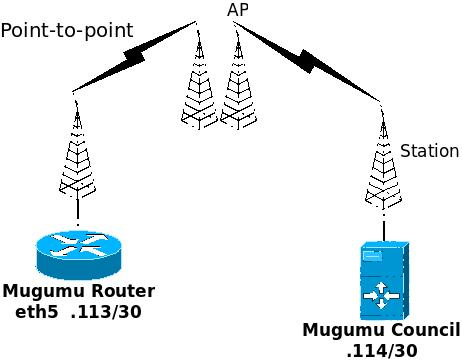
\includegraphics[width=\textwidth]{routed.jpeg}
\caption{Distribution of network with point-to-point link at Mugumu}
\label{ptp}
\end{subfigure}
\caption{Wireless Distribution System}
\end{figure}

Hence, it is proposed to set up a separate point-to-point link between fiber station and access point, which result in a topology in Figure \ref{ptp}. The point-to-point link is preferably operating in 5GHz domain to minimize inteference.

\subsection{Power Circuit Failure}
We observe occasional abnormal boot while testing Odroid router. When the system is recovered from power failure, Odroid platform sometimes, however, refuses to boot even though blue led (power light) is on, unless power pin is plugged out and back. The issue is yet to be investigated in laboratory.

\subsection{Network Monitoring and Administration}
To manage the system more efficiently, monitoring tools are yet to be deployed in the routers and other devices. There exist several Network Operations Centers in DIT, TERNET and KTH. Zabbix is deployed at some parts of the system although the installation is still incomplete. The task of configuring monitoring system propoerly is left to future work.